% This chapter should describe what was actually produced: the programs which were written, the hardware which was built or the theory which was developed. Any design strategies that looked ahead to the testing stage should be described in order to demonstrate a professional approach was taken.

% The repository overview should be around one page in length and should describe the high-level structure of the source code found in your source code repository. It should describe whether the code was written from scratch or if it built on an existing project or tutorial.

% Contribution to the field, with genuine potential for impact outside the tripos.

% Challenging goals and substantial deliverables, all methods and tools deployed expertly.

% Original techniques or methodologies going beyond what was previously known.

% Presentation is clear and concise throughout, with creative use of figures or diagrams.

% Excellent repository overview, giving clear insight into project structure.

\label{sec:3}

\section{Architectural Overview}
\label{sec:architectural-overview}

\begin{figure}[h]
    \centering
    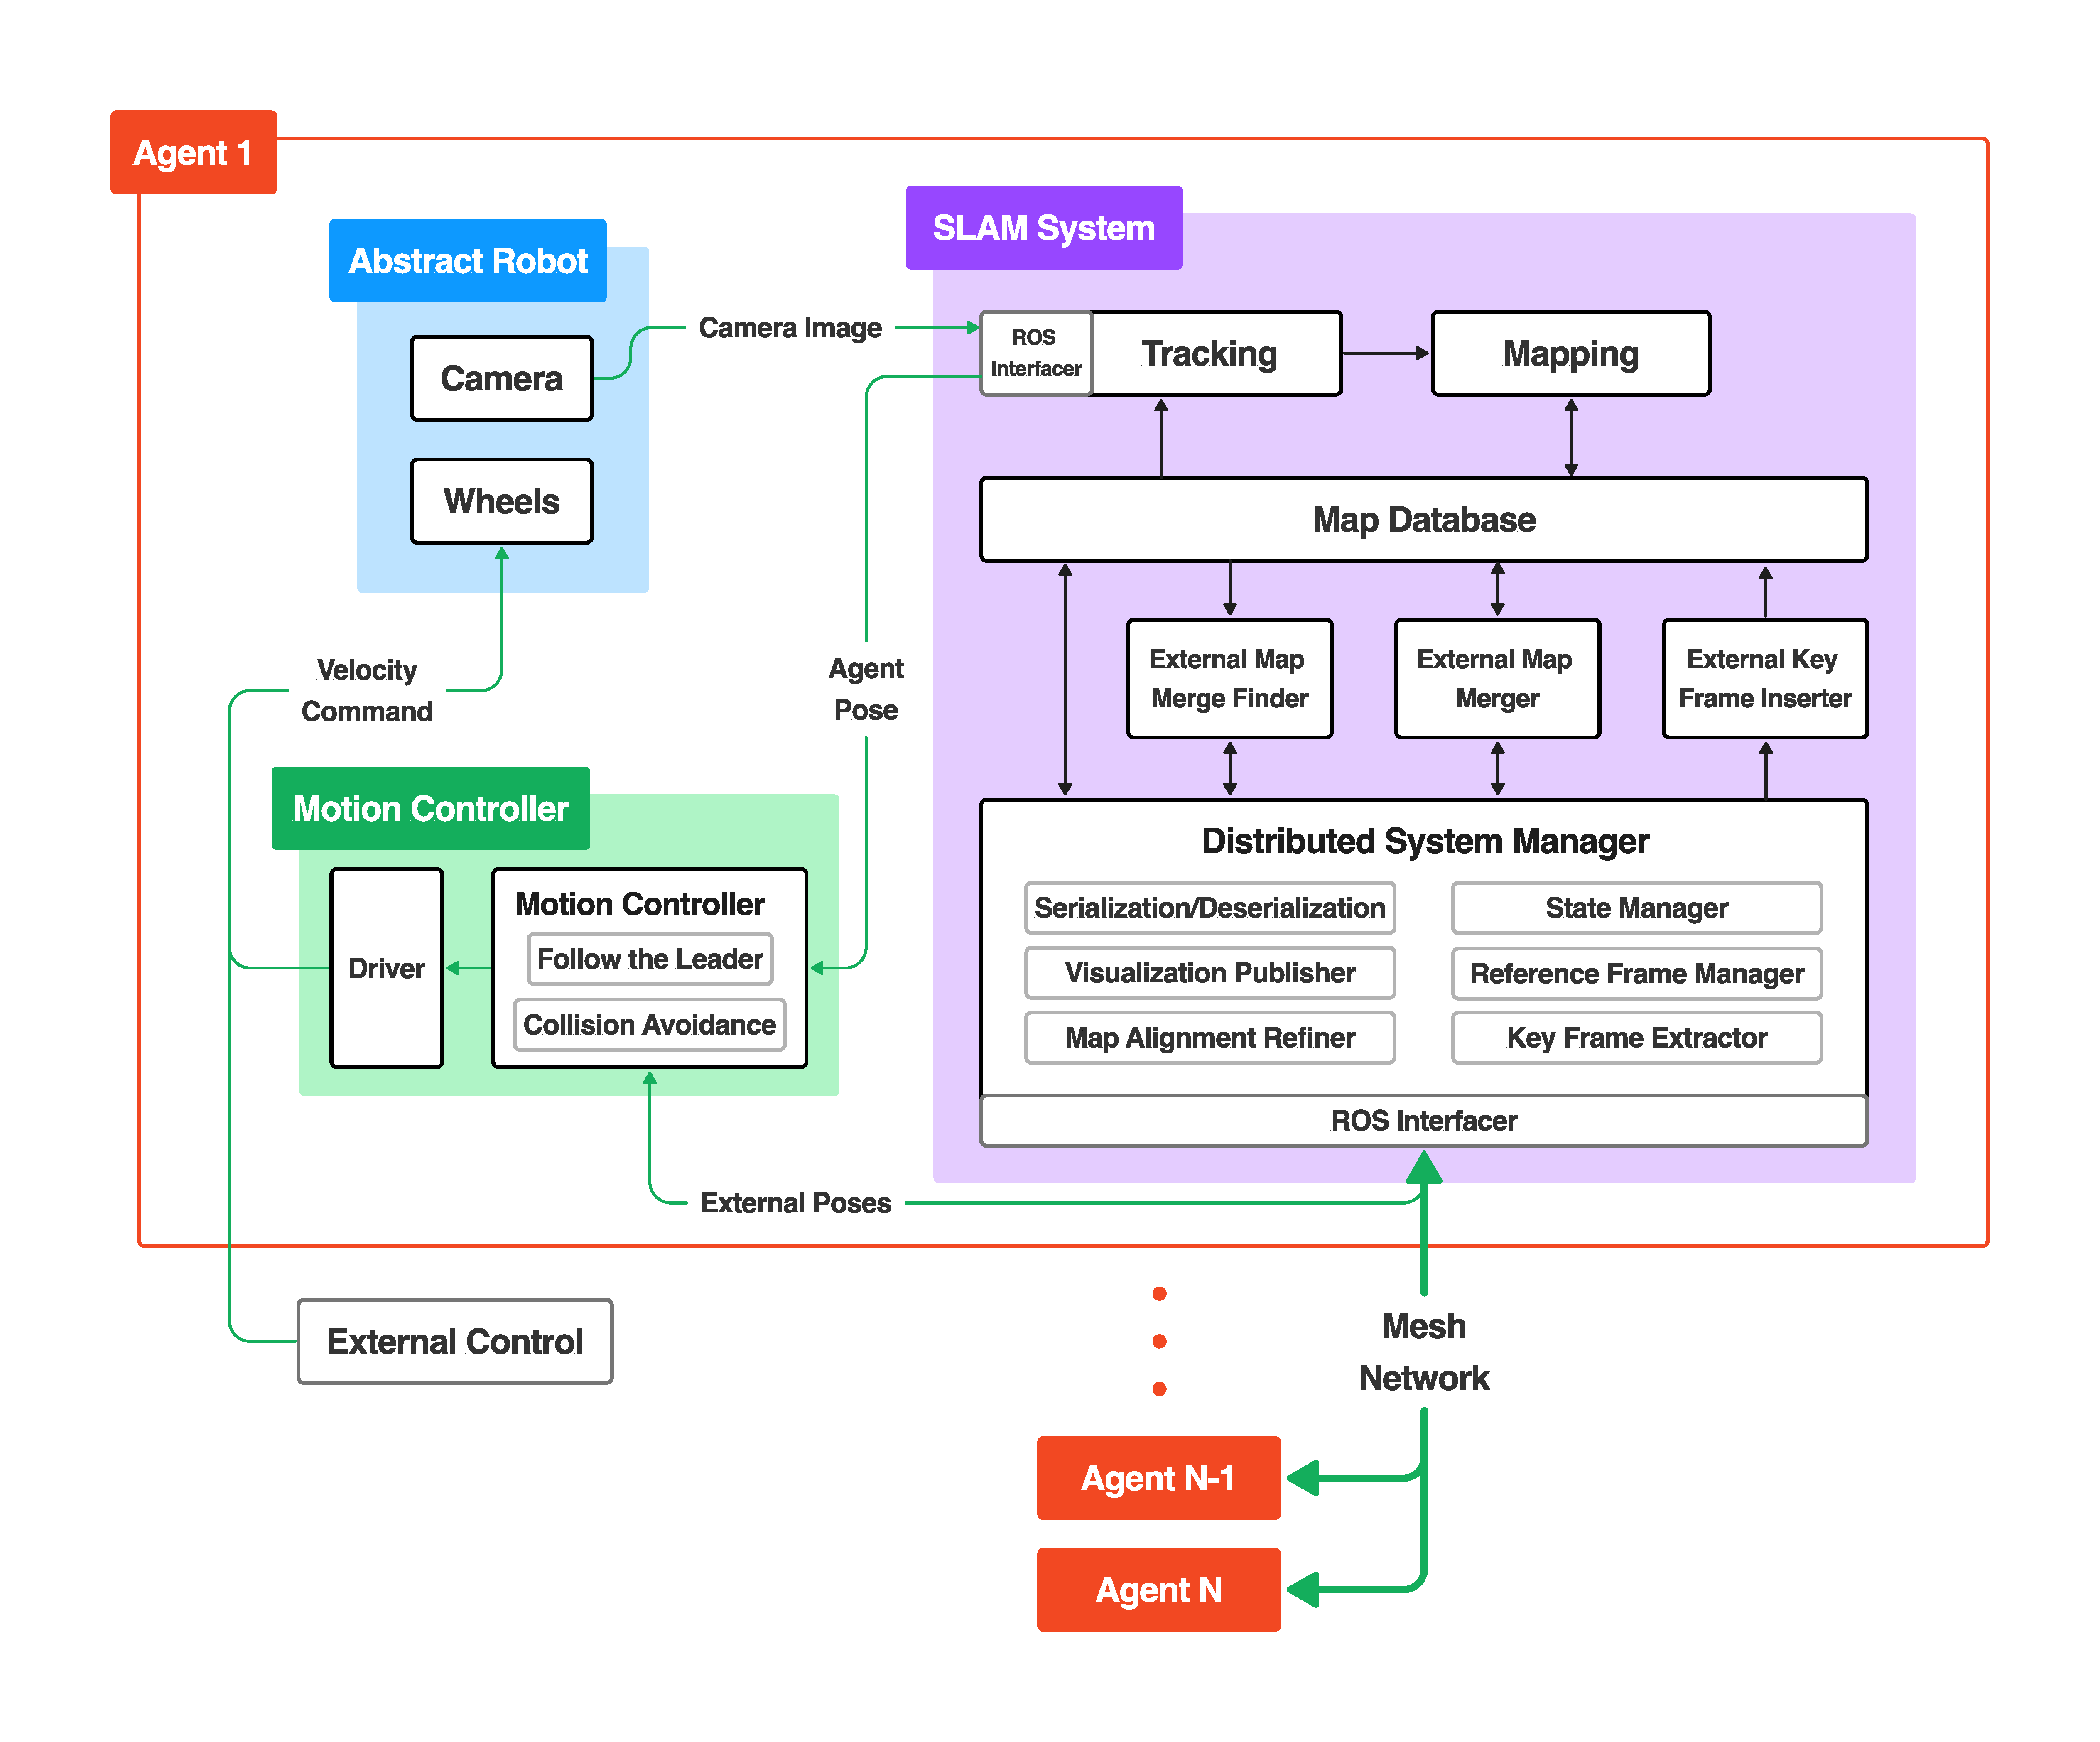
\includegraphics[trim=5cm 5cm 5cm 5cm, scale=0.2]{figures/agent_diagram.pdf}
    \caption{Agent diagram.}
    \label{fig:agent-diagram}
\end{figure}

\subsection{Repository Overview}
\label{sec:repository-overview}

\section{Simulation Environment}
\label{sec:simulation-environment}

\section{SLAM System}
\label{sec:slam-system}

\begin{figure}[h]
    \centering
    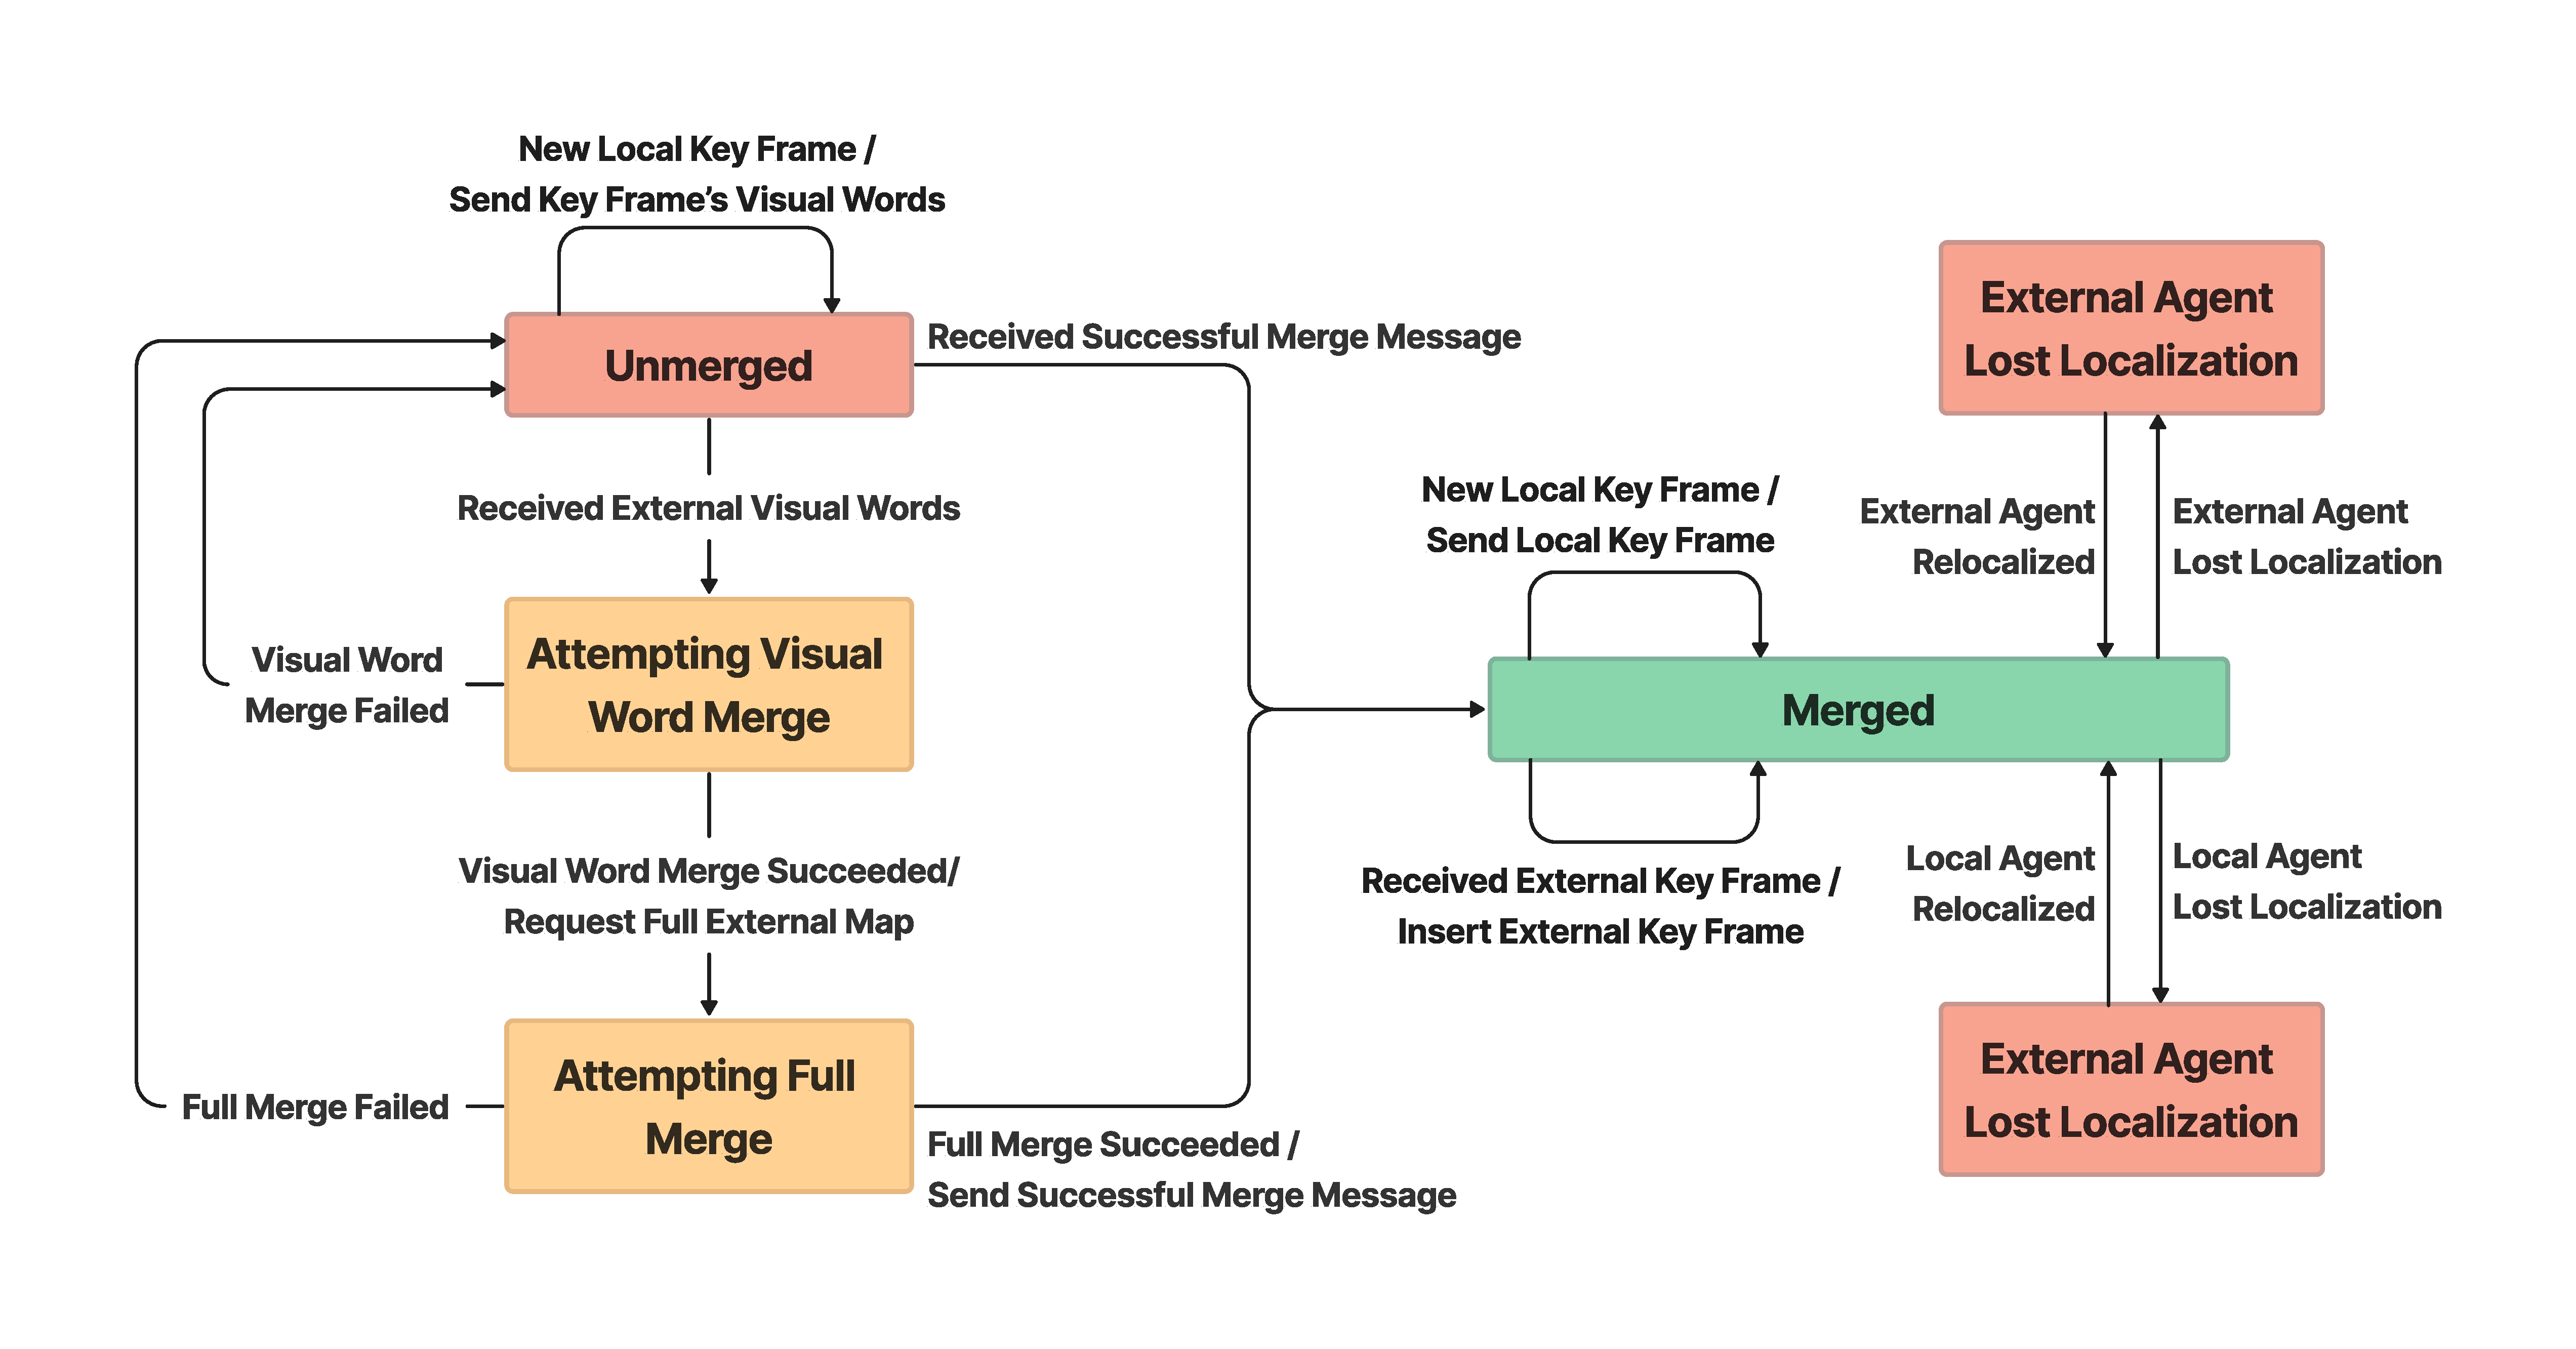
\includegraphics[trim=5cm 5cm 5cm 5cm, scale=0.2]{figures/slam_system_state_machine.pdf}
    \caption{SLAM system state machine for a single peer.}
    \label{fig:agent-diagram}
\end{figure}

\subsection{Distributed System Manager}
\label{sec:distributed-system-manager}

\subsubsection{State Manager}
\label{sec:state-manager}

\subsubsection{Map Alignment Refiner}
\label{sec:map-alignment-refiner}

\subsubsection{Reference Frame Manager}
\label{sec:reference-frame-manager}

\subsubsection{Visualization Publisher}
\label{sec:visualization-publisher}

\subsection{Map Serialization and Deserialization}
\label{sec:map-serialization-and-deserialization}

\subsection{External Map Merge Finder}
\label{sec:external-map-merge-finder}

\subsection{External Map Merger}
\label{sec:external-map-merger}

\subsection{External Key Frame Inserter}
\label{sec:external-key-frame-inserter}

\subsection{Keeping Coordinate Frames Consistant}
\label{sec:keeping-coordinate-frames-consistant}

\section{Motion Controller}
\label{sec:motion-controller}

\subsection{Follow The Leader}
\label{sec:follow-the-leader}

\subsection{Multi-Agent Collision Avoidance}
\label{sec:multi-agent-collision-avoidance}

\section{Custom Evaluation Suite – Multi-Agent EVO}
\label{sec:multi-agent-evo}
While there are several mature single-agent SLAM evaluation tools, I found there to be a complete lack of evaluation tools for multi-agent SLAM systems. Therefore, I have developed an open-source multi-agent SLAM evaluation tool: \textit{Multi Agent EVO}, based on the popular single agent SLAM evaluation tool \textit{EVO} \autocite{grupp2017evo}.

Besides the simple data structure and data ingestion modifications needed to allow EVO to process multi-agent SLAM data, there is some additional nuance to evaluating data from multiple agents.

Initially, all agents will be in separate reference frames until they explore an area previously seen by another agent, allowing them to merge their maps and share the same coordinate frame. We may also have cases where two independent groups of agents meet and merge maps, which requires multiple agents to simultaneously change coordinate frames. We also must note that these coordinate frames are part of the SIM(3) transformation group, which is composed of rotation, translation, and uniform scale in 3-dimensional space (scale being necessitated by the scale ambiguity of monocular visual SLAM).

Therefore, I have created a new data format to capture these changes in coordinate frames over time within our trajectory data, which Multi-Agent EVO is able to ingest. This allows us to properly compare the multi-agent SLAM trajectories to the ground truth data, giving us insights on how long it takes for agents to successfully merge maps, the accuracy of relative pose estimation, and much more.

TODO: add graph illustrating this coordinate frame stuff
TODO: perhaps list out all capabilities added

\section{Real World Implementation}
\label{sec:real-world-implementation}





